\PassOptionsToPackage{dvipsnames,svgnames,table}{xcolor}
\documentclass[11pt]{article}
\usepackage[a4paper,margin=22mm]{geometry}
\usepackage[no-math]{fontspec}
\setmainfont{DejaVu Serif}
\usepackage{amsmath,amssymb,amsthm,mathtools,graphicx,xcolor,hyperref,xurl,xspace,ifthen,enumerate}
\usepackage[shortlabels]{enumitem}
\setlength{\emergencystretch}{4em}
\AtBeginDocument{\special{pdf:mapline pzdr Dingbats <uzdr.pfb}}
\SetMathAlphabet{\mathbf}{normal}{OT1}{cmr}{bx}{n}
\SetMathAlphabet{\mathbf}{bold}{OT1}{cmr}{bx}{n}
\newtheorem{theo}{Theorem}[section]
\newtheorem{lemm}[theo]{Lemma}
\newtheorem{thm}[theo]{Theorem}
\newtheorem{proposition}[theo]{Proposition}
\newtheorem{corollary}[theo]{Corollary}
\newtheorem{definition}[theo]{Definition}
\newtheorem{theorem}[theo]{Theorem}
\newtheorem*{remas*}{Remarks}
\newtheorem{remas}[theo]{Remarks}
\newtheorem*{exam*}{Example}
\newtheorem{ques}[theo]{Question}
\providecommand{\og}{«\nobreakspace}
\providecommand{\fg}{\nobreakspace»}
\newtheorem{lem}[theo]{Lemma}
\newtheorem{lemma}[theo]{Lemma}
\newtheorem{prop}[theo]{Proposition}
\newtheorem{coro}[theo]{Corollary}
\newtheorem{corol}[theo]{Corollary}
\newtheorem*{conj*}{Conjecture}
\newtheorem{conj}[theo]{Conjecture}
\newtheorem{conjecture}[theo]{Conjecture}
\newtheorem{Proposition}[theo]{Proposition}
\newtheorem{theoreme}[theo]{Theorem}
\theoremstyle{definition}
\newtheorem{defi}[theo]{Definition}
\newtheorem{exam}[theo]{Example}
\newtheorem{exem}[theo]{Example}
\newtheorem{remark}[theo]{Remark}
\newtheorem{example}[theo]{Example}
\newtheorem{exams}[theo]{Examples}
\newtheorem{rema}[theo]{Remark}
\newtheorem{nota}[theo]{Notation}
\newtheorem{notation}[theo]{Notation}
\newtheorem*{notas}{Notations}
\newtheorem{result}[theo]{Result}
\newtheorem{question}[theo]{Question}
\newtheorem{prob}[theo]{Problem}
\newtheorem*{rema*}{Remark}
\newtheorem*{defi*}{Definition}
\newtheorem*{theo*}{Theorem}
\newtheorem*{lemm*}{Lemma}
\newtheorem*{prop*}{Proposition}
\newcommand{\enoncename}{}
\newtheorem{corpusenonce}[theo]{\enoncename}
\newenvironment{enonce}[2][]{\renewcommand{\enoncename}{#2}\begin{corpusenonce}}{\end{corpusenonce}}
\newenvironment{enonce*}[2][]{\par\medskip\noindent\textbf{#2.}\itshape}{\par\medskip}
\newenvironment{proofc}[1][\proofname]{\begin{proof}[#1]}{\end{proof}}
\newcommand{\Mc}{\mathcal{M}}
\newcommand{\pointir}{.\ ---\ }
\newcommand{\equalenv}[2]{\expandafter\let\csname#1\expandafter\endcsname\csname#2\endcsname\expandafter\let\csname end#1\expandafter\endcsname\csname end#2\endcsname}
\providecommand{\diagbox}[3][]{\begin{tikzpicture}[x=1em,y=1em,baseline=(current bounding box.center)]\useasboundingbox(0,0) rectangle(3,1.4);\draw(0,1.4)--(3,0);\node at(.5,.3){#2};\node at(2.5,1.1){#3};\end{tikzpicture}}
\providecommand{\eg}{e.g.\ }
\providecommand{\ie}{i.e.\ }
\providecommand{\cf}{cf.\ }
\providecommand{\longthanks}[1]{\par\smallskip\noindent #1\par\smallskip}
\providecommand{\qbinom}[2]{\genfrac{[}{]}{0pt}{}{#1}{#2}}

\providecommand{\mathof}[1]{\mathrm{#1}}

\numberwithin{equation}{section}


\def\endappendix{}


\usepackage{latexsym,amsmath,amssymb,verbatim,tikz,tikz-cd}
\usepackage{mathtools}
\usepackage{graphicx,xcolor}

\usepackage[english]{babel}
\usepackage{amssymb}
\usepackage{amsmath}
\usepackage{amsthm}
\usepackage{graphicx}
\usepackage{csquotes}
\usepackage{bm}
\usepackage{enumitem}
\usepackage{subcaption}
\usepackage{caption}
\renewcommand{\thesubfigure}{\Alph{subfigure}}
\usepackage{dirtytalk}
\providecommand{\nopunct}{\spacefactor1007\relax}
\newtheorem{problem}[theo]{Problem}

\newcommand{\sym}{\mathrm{Sym}}
\newcommand{\qsym}{\mathrm{QSym}}
\newcommand{\Des}{\operatorname{Des}}
\newcommand{\Asc}{\operatorname{Asc}}
\newcommand{\Syt}{\operatorname{SYT}}
\newcommand{\Short}{\operatorname{Short}}
\newcommand{\Loop}{\operatorname{Loop}}
\newcommand{\Stable}{\operatorname{Stable}}
\newcommand{\len}{\operatorname{len}}
\newcommand{\height}{\operatorname{height}}
\newcommand{\core}{\operatorname{core}}
\newcommand{\res}{\operatorname{res}}
\newcommand{\row}{\operatorname{row}}
\newcommand{\insrt}{\operatorname{insert}}
\newcommand{\UP}{\operatorname{UP}}
\newcommand{\DOWN}{\operatorname{DOWN}}


\newcommand{\ZZ}{\mathbb{Z}}
\newcommand{\NN}{\mathbb{N}}
\newcommand{\RR}{\mathbb{R}}
\newcommand{\QQ}{\mathbb{Q}}
\newcommand{\PP}{\mathbb{P}}

\newcommand{\F}{\mathcal{F}}
\newcommand{\Q}{\mathcal{Q}}
\newcommand{\A}{\mathcal{A}}
\newcommand{\M}{\mathcal{M}}
\newcommand{\I}{\mathcal{I}}
\newcommand{\PM}{\mathcal{PM}}
\newcommand{\Pcal}{\mathcal{P}}


\newcommand{\odds}{\mathrm{odds}}

\makeatletter
\newcommand{\proofstep}[1]{
  \par
  \addvspace{\medskipamount}
  \textbf{#1\@addpunct{.}}\enspace\ignorespaces
}

\newcommand\restr[2]{{
  \left.\kern-\nulldelimiterspace 
  #1 
  \vphantom{\big|} 
  \right|_{#2} 
  }}
\makeatother












% Presentation adapter only; author mathematics is unchanged.
% Original packages: alco-351-publisher.tex lines 3-4, retained verbatim.
\usepackage{ytableau,shuffle}
\usepackage[enableskew,vcentermath]{youngtab}
% Original line 88: \newtheorem{observation}[cdrthm]{Observation}
% cedram counter cdrthm is replaced by existing AMS wrapper counter theo.
\newtheorem{observation}[theo]{Observation}
\usepackage{needspace}
\title{Schur expansion of matchings with fixed unmatched-vertex count via the core-tableau bijection}
\author{Avichai Marmor}
\date{doi:10.5802/alco.351; CC BY 4.0}
\begin{document}
\maketitle
\noindent\textit{Editorial note.} In the retained publisher source, the theorem statement and the bijection target use upper bound n, with N = 2n + f. The displayed summation in the final concluding proof instead prints upper bound N (source line 1018). This discrepancy is retained verbatim; this note is editorial and does not replace or amend the author formula.\par\medskip
\noindent\textit{Editorial note.} Source674-980 was displayed as context in the older package but explicitly reviewed as a carrying proof obligation. Its role is now proof; the original excerpt and mathematical scope are retained.\par\medskip
\noindent\textit{Editorial note.} The original reviewer resolved the empty stable-set boundary by the already-stated noncrossing-removal property on the entire interval. No convention for invalid or negative tableau sizes is introduced.\par\medskip
\noindent\textit{Editorial scope.} One counted theorem: the matching Schur expansion through the full stable-core/two-row-SYT/ballot bijection. The public Theorem1.8 is not a free prerequisite. The alternate first proof and rejected Knuth-only task are not separately counted.\par\medskip
\noindent\textit{Allowed standard prerequisites (editorial).}\begin{itemize}
\item Gessel fundamental-quasisymmetric expansion of Schur functions over SYT. Publisher source361-364, retained in the standard-input context.. Apply only after the full Short=Des bijection is proved.
\item Adin-Roichman descent-statistic criterion. Publisher source366-376, retained in the standard-input context.. The declared classical Schur-theoretic criterion; same-paper Theorem1.8 is NOT a free input.
\end{itemize}\medskip
\section{Introduction}
\label{sec:introduction}

Denote the set of nonnegative integers by $\NN$, and the set of positive integers by $\PP$. Given $N\in \NN$ and a set $\A$, together with a set-valued function $D:\A\to 2^{[N-1]}$ which is sometimes called a \emph{statistic}, we define its quasisymmetric generating function
\[
    \Q_{D} (\A) = \sum_{a \in \A} F_{N, D(a)},
\]
where $F_{N, S}$ is the \emph{fundamental quasisymmetric function} introduced by Gessel~\cite{knuth_classes_schur_positive}, indexed by a subset $S \subseteq [N-1]$ (see Section~\ref{subsec:definitions symmetric functions} for more background). We write $\Q(\A)$ instead of $\Q_{D}(\A)$ when $D$ is clear from the context.
The following long-standing problem was first addressed in~\cite{gessel1993counting}.
\begin{problem}[Gessel and Reutenauer]
    Find sets $\A$ and statistics $D$ for which $\Q_{D}(\A)$ is symmetric.
\end{problem}

When $\Q_{D}(\A)$ is symmetric, we say that $\A$ is symmetric with respect to the statistic $D$ (we omit $D$ when it is clear from the context). If $\A$ is symmetric, then there is a unique expansion
\[
    \Q_{D} (\A) = \sum_{\lambda \vdash N} c_\lambda s_\lambda,
\]
where $c_\lambda \in \QQ$ and $s_\lambda$ are Schur functions (discussed in Section~\ref{subsec:definitions symmetric functions}). The coefficients $c_\lambda$ are called the \emph{Schur coefficients} of $\A$.
If $c_\lambda \in \NN$ for all $\lambda \vdash N$, we say that $\A$ is Schur-positive with respect to $D$.

\begin{definition}
\label{def:matching}
    A matching $m$ on a finite set of vertices $S \subseteq \PP$ is an unordered partition of $S$ into blocks, each block of size $1$ or $2$. If a block of a matching $m$ contains only the vertex $i$, we say that $i$ is an \emph{unmatched vertex} of $m$ and denote $(i) \in m$. If a block contains both $i$ and $j$ for $i<j$, we say that $(i,j)$ is a \emph{chord} of $m$ and denote $(i,j) \in m$. That is, the notation $(i,j)\in m$ implies that $i<j$. When $(i,j) \in m$, we also say that $i$ opens this chord and $j$ closes it. If a matching $m$ has no unmatched vertex, then we say that $m$ is a perfect matching.
\end{definition}

We will focus on matchings on the set $[N] := \{1,\dots, N\}$ for some $N \in \NN$. Denote by $\M_N$ the set of matchings on $[N]$, and by $\M_{N,f}$ the set of matchings on $[N]$ with $f$ unmatched vertices.

For example, 
\[
    \M_{4,0} = \big\{\{(1,2),\; (3,4)\},\ \{(1,3),\; (2,4)\},\ \{(1,4),\; (2,3)\}\big\}
\]
and
\[ 
    \M_{3,1} = \big\{\{(1,2),\; (3)\},\ \{(1,3),\; (2)\},\ \{(1),\; (2,3)\}\big\}.
\]

\begin{definition}
\label{def:intersect}
    Let $m$ be a matching on $S$. If $(i_1, i_3),\: (i_2,i_4) \in m$ for $i_1 < i_2 < i_3 < i_4$ then we say that the chords $(i_1, i_3)$ and $(i_2, i_4)$ \emph{intersect}.
\end{definition}

\begin{definition}
\label{def:short}
    Let $m \in \M_N$ be a matching on $[N]$. If $(i,i+1) \in m$, then it is called a \emph{short chord}. We denote $\Short(m) := \{i \in [N-1] \mid (i,i+1) \in m\}$.

\end{definition}

For example, consider the matching $m = \{(1,3),\; (2,6),\; (4,5)\}$ as in Figure~\ref{fig:matching example introduction}. In this matching the chords $(1,3)$ and $(2,6)$ intersect, and $\Short(m) = \{4\}$ (since $(4,5) \in m$).
\begin{figure}[htb]
    \begin{center}
        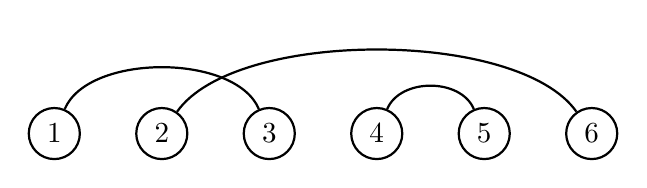
\begin{tikzpicture}[node distance={13mm}, thick, main/.style = {draw, circle, scale=1.05}]  
            \node[main] (1) {$1$};
            \node[main] (2) [right of=1] {$2$};
            \node[main] (3) [right of=2] {$3$};
            \node[main] (4) [right of=3] {$4$};
            \node[main] (5) [right of=4] {$5$};
            \node[main] (6) [right of=5] {$6$};
            
            
            \draw (1) to [out=67,in=113,looseness=0.8] (3);
            \draw (2) to [out=55,in=125,looseness=0.65] (6);
            \draw (4) to [out=67,in=113,looseness=1] (5);
        \end{tikzpicture}
    \end{center}
    \caption{The matching $m = \{(1,3),\; (2,6),\; (4,5)\}$.}
    \label{fig:matching example introduction}
\end{figure}

Note that $N \notin \Short(m)$ for every $m \in \M_N$. This holds even where $(1,N) \in m$.

\begin{theorem}
\label{thm:matchings schur positive}
    Let $n,f \in \NN$ be nonnegative integers, and denote $N=2n+f$. Then the set $\M_{N,f}$ is Schur-positive with respect to $\Short$. Furthermore, its Schur expansion is given by the following formula:
    \[
        \Q_{\Short} (\M_{N,f}) = \sum_{k=0}^n |\{ m\in \M_{N-2k,f} \mid \Short(m) = \emptyset\}|\ s_{N-k,k}.
    \]
\end{theorem}

\section{Preliminaries and notation}
\label{sec:preliminaries}

\begin{definition}
    For nonnegative integers $i,j$, we define the \emph{interval}
    \[
        [i,j] :=
        \begin{cases}
            \{i,i+1,\dots,j\} & \text{if $i \le j$,}\\
            \emptyset & \text{otherwise.}
        \end{cases}
    \]
    We also define $[i] = [1,i]$.
\end{definition}

\begin{definition}
\label{def:elements with given stat}
    Given a set $\A$, a function $D:\A \to 2^{[N-1]}$ and a set $J \subseteq [N-1]$, we denote $\A(D=J) := \{a \in \A \mid D(a) = J\}$ and $\A(D \supseteq J) := \{a \in \A \mid D(a) \supseteq J\}$.
\end{definition}

\subsection{Symmetric and quasisymmetric functions}
\label{subsec:definitions symmetric functions}

\begin{definition}
    Given $N \in \NN$, a \emph{partition} $\lambda$ of $N$ (denoted $\lambda \vdash N$), is a weakly-decreasing sequence $\lambda = (\lambda_1 \ge \lambda_2 \ge \dots \ge \lambda_\ell)$ of positive integers, such that $\lambda_1 + \dots + \lambda_\ell = N$. The values $(\lambda_1,\dots,\lambda_\ell)$ are called the \emph{parts} of $\lambda$.
    
    A \emph{composition} $\alpha$ of $N$ (denoted $\alpha \vDash N$) is a sequence $\alpha = (\alpha_1, \alpha_2, \dots, \alpha_\ell )$ of positive integers, such that $\alpha_1 + \dots + \alpha_\ell = N$. Every partition is a composition.
\end{definition}

Compositions of $N$ are in bijection with subsets of $[N-1] := \{1, \dots, N-1\}$ by 
\[
    [N-1] \supseteq \{i_1, i_2, \dots, i_\ell \} \mapsto (i_1, i_2 - i_1, \dots, i_\ell - i_{\ell-1}, N - i_\ell) \vDash N.
\]
For example, for $N = 10$, $\{2, 4, 7, 8\} \mapsto (2, 2, 3, 1, 2)$. The composition associated to a set $S$ is denoted $\alpha_S$, and the set associated to a composition $\alpha$ is denoted $S_\alpha$.

We say that two compositions $\alpha, \beta \vDash N$ are \emph{equivalent} (denoted $\alpha \sim \beta$), if $\beta$ is a rearrangement of the entries of $\alpha$.

Denote the ring of symmetric functions by $\sym$ and the ring of quasisymmetric functions by $\qsym$ (see, for example, \cite[Section 1]{S3_patterns_list} for details). The space of homogeneous symmetric functions of degree $N$ is denoted by $\sym_N$, and the space of homogeneous quasisymmetric functions of degree $N$ is denoted by $\qsym_N$.

The space $\qsym_N$ has several important bases. In this work, we focus on the \emph{fundamental basis}, consisting of the functions
\[
    F_{N,S} := \sum_{\substack{i_1 \le i_2 \le \dots \le i_N \\ \forall j \in S:i_j < i_{j+1}}} x_{i_1} x_{i_2} \dots x_{i_N},\quad S \subseteq [N - 1].
\]
We write $F_S$ instead of $F_{N,S}$ when $N$ is clear from the context.

The space $\sym_N$ has several standard bases as well. In this work, we focus on the Schur basis, which consists of the Schur functions $s_{\lambda}$, where $\lambda$ is a partition of $N$. 
The definition and properties of Schur functions can be found in \cite[Section 4.4]{sagan_book}. Here, we adopt the combinatorial approach to Schur functions, as described in Theorem~\ref{thm:schur functions young tableaux} and Theorem~\ref{thm:criterion schur positive young} below.

\subsection{Symmetric and Schur-positive sets}
\label{subsec:schur positive sets}
As mentioned in Section~\ref{sec:introduction}, a set $\A$ is symmetric with respect to a statistic $D:\A \to 2^{[N-1]}$ if the generating function $\Q_{D}(\A)$ is a symmetric function. Moreover, it is Schur-positive if all Schur coefficients are nonnegative integers.


One of the fundamental constructions of Schur-positive sets, regarding sets of standard Young tableaux (SYT), is due to Gessel~\cite{knuth_classes_schur_positive}. Let $\Syt(\lambda)$ denote the set of standard Young tableaux of shape $\lambda$. We draw tableaux in English notation, as in Figure~\ref{fig:SYT example}. The \emph{descent set} of $T\in \Syt(\lambda)$ is
\[
    \Des(T) := \{i \in [N-1] \mid i+1 \text{ appears in a lower row than $i$ in $T$}\}.
\]
For example, the descent set of the SYT in Figure~\ref{fig:SYT example} is $\{2,4,7,8\}$.

\begin{figure}[htb]
	\[
            \young(1247,36,58,9)
        \]
	\caption{A SYT of shape $\lambda = (4,2,2,1)$.} 
	\label{fig:SYT example}
\end{figure}

The entry in row $i$ and column $j$ of a tableau $T \in \Syt(\lambda)$ is denoted by $T_{i,j}$. In addition, we define $\row_i(T) := \{T_{i,j} \mid 1 \le j \le \lambda_i\}$ as the set of entries in the $i$-th row of $T$. For example, if we consider the SYT shown in Figure~\ref{fig:SYT example}, then $T_{3,2} = 8$ and $\row_3(T) = \{5,8\}$.

\begin{theorem}[Gessel~\cite{knuth_classes_schur_positive}]
\label{thm:schur functions young tableaux}
    For every $\lambda \vdash N$, the set $\Syt(\lambda)$ is Schur-positive with respect to $\Des$. Moreover, $\Q(\Syt(\lambda)) = s_\lambda$.
\end{theorem}

In 2015, Adin and Roichman proved the following criterion.
\begin{theorem}[{\cite[Prop.\ 9.1]{adin_roichman_fine_set}}]
\label{thm:criterion schur positive young}
    A set $\A$ is symmetric with respect to $D:\A\to 2^{[N-1]}$ if and only if
    \[
        \sum_{a \in \A} \boldsymbol{t}^{D(a)} = \sum_{\lambda \vdash N} c_\lambda \sum_{T \in \Syt(\lambda)} \boldsymbol{t}^{\Des(T)}
    \]
    for some values $c_\lambda$, where $\boldsymbol{t}^J := \prod_{j \in J} t_j$ for $J \subseteq [N-1]$. The coefficients $c_\lambda$ are the Schur-coefficients of $\A$. Moreover, $\A$ is Schur-positive if and only if $c_{\lambda} \in \NN$ for all $\lambda \vdash N$.
\end{theorem}

This criterion implies that proving the Schur-positivity of a set is achievable by establishing a statistic-preserving bijection between the set and SYTs of shapes corresponding to a specific multiset.

\subsection{Bijective proof of Theorem~\ref{thm:matchings schur positive}}
\label{subsec:bijective proof matchings schur positive}

Before presenting the bijective proof of Theorem~\ref{thm:matchings schur positive}, we give some definitions and notations for matchings:






\begin{definition}
\label{def:restriction of matching}
    Given a matching $m \in \M_N$, we say that a set $S \subseteq [N]$ is $m$-invariant if for every chord $(i,j) \in m$ we have $i \in S$ if and only if $j \in S$. Moreover, for a matching $m$ and an $m$-invariant set $S$ we define the \emph{restriction} of $m$ to $S$, denoted $\res_S(m)$, to be a matching on $S$ which is obtained by removing all the vertices not in $S$ from $m$.
\end{definition}

For example , consider the matching $m_1 = \{(1,2),\; (3,5),\; (4)\} \in \M_{5,1}$ as in Figure~\ref{fig:core first example before}. The set $S_1=\{1,2,4\}$ is $m_1$-invariant, and $\res_{S_1}(m_1)=\{(1,2),\; (4)\}$. On the other hand, the set $S_2 = \{1,2,3\}$ is not $m_1$-invariant, so $\res_{S_2}(m_1)$ is not defined.


\begin{observation}
\label{obs:restriction of matching to set and complement defines uniquely}
    Let $S \subseteq [N]$ be a set of vertices, let $m_1$ be a matching on $S$, and let $m_2$ be a matching on $[N]\setminus S$. Then there exists a unique matching $m \in \M_N$ such that $\res_S(m) = m_1$ and $\res_{[N] \setminus S}(m) = m_2$.
\end{observation}


Now let us present a bijection
\[
    F:\M_{N,f} \to \bigcup_{k=0}^n \M_{N-2k,f}(\Short = \emptyset) \times \Syt(N-k,k),
\]
that sends matchings $m \in \M_{N,f}$ to pairs $(m_0,T)$, where $m_0$ is a short-chord-free matching on $[N-2k]$ with $f$ unmatched vertices and $T\in \Syt(N-k,k)$ for some $0\le k \le n$, such that
$\Des T = \Short m$ for all $m$. By Theorem~\ref{thm:criterion schur positive young}, the existence of such a bijection implies Theorem~\ref{thm:matchings schur positive}.

\subsubsection{Constructing the bijection}
\label{subsec:constructing the bijection}
First, we define the core of a matching:
\begin{definition}
\label{def:core of matching}
    The reduction process for a given matching $m$ repeatedly removes any short chords of the matching until there are no short chords left. The remaining vertices are then re-indexed with natural numbers starting from $1$ while keeping their relative order, resulting in a matching denoted by $\core(m)$.
    
    A chord or vertex of $m$ is called \emph{stable} if it is not removed during the process, and unstable otherwise.
    The set of stable vertices of $m$ is denoted $\Stable(m)$.
\end{definition}

Proposition~\ref{prop:core well defined} below implies that $\core(m)$ and $\Stable(m)$ are well-defined and are independent of the order of the steps.

For a matching $m \in \M_{N,f}$, we also define $T(m)$ as the unique SYT consisting of $N$ cells arranged in two rows, such that
\[
    \row_2(T) = \{j \mid \text{the chord } (i,j) \in m \text{ is unstable}\}.
\]
Recall that when writing $(i,j) \in m$ we assume that $i<j$. Therefore, for every unstable chord $(i,j)\in m$ with $i<j$, we have $i \in \row_1(T(m))$ and $j \in \row_2(T(m))$. We define the bijection by $F(m) = (\core(m),T(m))$.

Next, we turn to provide examples of the bijection. Then, in the remaining of the subsection, we will prove that the bijection is well-defined and explore some of its properties. Section~\ref{subsec:proof of bijection} will be devoted to proving that $F$ is bijective by constructing its inverse function.

As a first example, consider the matching $m_1 = \{(1,2),\; (3,5),\; (4)\} \in \M_{5,1}$ as in Figure~\ref{fig:core first example before}.

\begin{figure}[htb]
    \begin{subfigure}{\textwidth}
        \begin{center}
            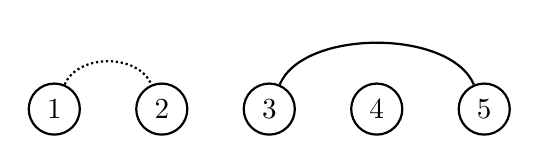
\begin{tikzpicture}[node distance={13mm}, thick, main/.style = {draw, circle, scale=1.05}]  
                \node[main] (1) {$1$};  
                \node[main] (2) [right of=1] {$2$}; 
                \node[main] (3) [right of=2] {$3$}; 
                \node[main] (4) [right of=3] {$4$}; 
                \node[main] (5) [right of=4] {$5$}; 
                
                \draw[densely dotted] (1) to [out=67,in=113,looseness=1] (2);  
                \draw (3) to [out=67,in=113,looseness=0.8] (5);
            \end{tikzpicture}
        \end{center}
        \caption{Plot of $m_1$}
        \label{fig:core first example before}
    \end{subfigure}
    \begin{subfigure}{\textwidth}
        \begin{center}
            \vspace{3ex}
            \begin{subfigure}{0.3\textwidth}
                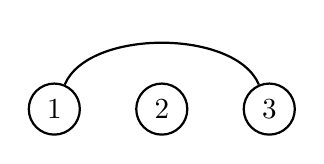
\begin{tikzpicture}[node distance={13mm}, thick, main/.style = {draw, circle, scale=1.05}]  
                    \node[main] (1) {$1$};  
                    \node[main] (2) [right of=1] {$2$}; 
                    \node[main] (3) [right of=2] {$3$}; 
                    
                    \draw (1) to [out=67,in=113,looseness=0.8] (3);
                \end{tikzpicture}
            \end{subfigure}
            \begin{subfigure}{0.2\textwidth}
                \[
                    \young(1345,2)
                \]
                \vspace{0.1ex}
            \end{subfigure}
        \end{center}
        \caption{Plot of $\core(m_1)$ and $T(m_1)$}
        \label{fig:core first example core}
    \end{subfigure}
    \caption{Example of the bijection for the matching $m_1 = \{(1,2),\; (3,5),\; (4)\} \in \M_{5,1}$}
    \label{fig:core first example}
\end{figure}

            
            
            
            

During the reduction process of $m_1$, the short chord $(1,2)$ is removed. Then, the vertices $3,4,5$ remain, so $\Stable(m_1) = \{3,4,5\}$. Next, the stable vertices are renumbered to $\{1,2,3\}$, so $\core(m_1) = \{(1,3),\; (2)\}$, as in Figure~\ref{fig:core first example core}. In addition, the only unstable chord of $m_1$ is $(1,2)$, so $\row_2(T(m_1))=\{2\}$. Therefore, $T(m_1)$ is the tableau presented in Figure~\ref{fig:core first example core}.

Next, consider the matching $m_2 = \{(1,7),\; (2,10),\; (3,6),\; (4,5),\; (8,9)\} \in \M_{10,0}$ as in Figure~\ref{fig:core second example before}.

\begin{figure}[htb]
    \begin{subfigure}{\textwidth}
        \begin{center}
            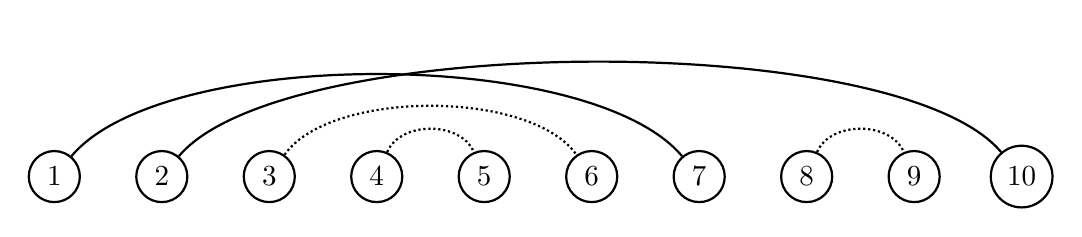
\begin{tikzpicture}[node distance={13mm}, thick, main/.style = {draw, circle, scale=1.05}]  
            \node[main] (1) {$1$};
            \node[main] (2) [right of=1] {$2$};
            \node[main] (3) [right of=2] {$3$};
            \node[main] (4) [right of=3] {$4$};
            \node[main] (5) [right of=4] {$5$};
            \node[main] (6) [right of=5] {$6$};
            \node[main] (7) [right of=6] {$7$};
            \node[main] (8) [right of=7] {$8$};
            \node[main] (9) [right of=8] {$9$};
            \node[main] (10) [right of=9] {$10$};
            
            \draw (1) to [out=50,in=130,looseness=0.6] (7);
            \draw (2) to [out=50,in=130,looseness=0.5] (10);
            \draw[densely dotted] (3) to [out=55,in=125,looseness=0.7] (6);
            \draw[densely dotted] (4) to [out=67,in=113,looseness=1] (5);
            \draw[densely dotted] (8) to [out=67,in=113,looseness=1] (9);
        \end{tikzpicture}
        \end{center}
        \caption{Plot of $m_2$}
        \label{fig:core second example before}
    \end{subfigure}
    \begin{subfigure}{\textwidth}
        \begin{center}
            \vspace{3ex}
            \begin{subfigure}{0.4\textwidth}
                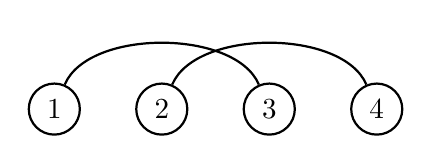
\begin{tikzpicture}[node distance={13mm}, thick, main/.style = {draw, circle, scale=1.05}]  
                    \node[main] (1) {$1$};  
                    \node[main] (2) [right of=1] {$2$}; 
                    \node[main] (3) [right of=2] {$3$}; 
                    \node[main] (4) [right of=3] {$4$}; 
                    
                    \draw (1) to [out=67,in=113,looseness=0.8] (3);
                    \draw (2) to [out=67,in=113,looseness=0.8] (4);
                \end{tikzpicture}
            \end{subfigure}
            \begin{subfigure}{0.4\textwidth}
                \[
                    \newcommand\ten{10}
                    \young(123478\ten,569)
                \]
                \vspace{0.1ex}
            \end{subfigure}
        \end{center}
        \caption{Plot of $\core(m_2)$ and $T(m_2)$}
        \label{fig:core second example core}
    \end{subfigure}
    \caption{Example of the bijection for the matching $m_2 = \{(1,7),\; (2,10),\; (3,6),\; (4,5),\; (8,9)\} \in \M_{10,0}$}
    \label{fig:core second example}
\end{figure}
            
            

            
            
            

During the reduction process of $m_2$, we first remove the short chords $(4,5)$ and $(8,9)$. Then, the chord $(3,6)$ becomes short and is subsequently removed as well. The remaining vertices are $1,2,7$ and $10$, so $\Stable(m_2) = \{1,2,7,10\}$. Next, the stable vertices are renumbered to $[4]$, so $\core(m_2) = \{(1,3),\; (2,4)\}$, as in Figure~\ref{fig:core second example core}. In addition, the unstable chords of $m_2$ are $(3,6),\; (4,5)$ and $(8,9)$, so $\row_2(T(m_2))=\{5,6,9\}$. Therefore, $T(m_2)$ is the tableau presented in Figure~\ref{fig:core second example core}.
            
            

Moving on to proving that the bijection $F$ is well-defined, first let us prove that the core of a matching is well-defined:

\begin{proposition}
\label{prop:core well defined}
    Given a matching, its stable vertices and its core are well-defined.
\end{proposition}
\begin{proof}
    Let $m \in \M_N$ be a matching. Denote the chords that are removed during a given reduction process of $m$ by $e_1, \dots, e_k$, and denote $e_\ell = (i_\ell,j_\ell)$. Moreover, denote the chords that are removed during another reduction process by $e_1', \dots, e_{k'}'$, and denote $e_\ell' = (i_\ell',j_\ell')$. It suffices to prove that $e_\ell \in \{e_1', \dots, e_{k'}'\}$ for all $1 \le \ell \le k$ (\ie every chord that is removed during the first reduction process is removed during the second process as well). Assume by contradiction that $e_\ell \notin \{e_1', \dots, e_{k'}'\}$ for some $\ell$, and denote by $\ell_0$ the minimal such $\ell$.
    That is, $e_1,\dots,e_{\ell_0-1} \in \{e_1', \dots, e_{k'}'\}$. Removing the chords $e_1, \dots, e_k$ from $m$ constitutes a valid reduction process, so the chord $e_{\ell_0}$ becomes short before it is removed. That is, $i \in \{i_1,j_1,\dots,i_{\ell_0-1},j_{\ell_0-1}\}$ for all $i_{\ell_0} < i < j_{\ell_0}$. Therefore, the chord $e_{\ell_0}$ is a short chord of the core obtained by removing $e_1', \dots, e_{k'}'$ of $m$, contradicting the requirement that the reduction process continues until there are no short chords remaining. Therefore, we may conclude that if a chord is removed during a reduction process then it is removed during any reduction process, and $\core(m)$ and $\Stable(m)$ are well-defined.
\end{proof}
\begin{corollary}
    Let $N$ and $f$ be nonnegative integers. Then the function
    \[
        F:\M_{N,f} \to \bigcup_{k=0}^n \M_{N-2k,f}(\Short = \emptyset) \times \Syt(N-k,k)
    \]
    defined by $F(m) = (\core(m),T(m))$ is well-defined.
\end{corollary}
\begin{proof}
    Let $m\in \M_{N,f}$ be a matching. By Proposition~\ref{prop:core well defined}, we obtain that $\core(m)$ and $\Stable(m)$ are well-defined. Therefore, the two-row tableau $T:=T(m)$ consisting of $N$ cells that is defined by
    \[
        \row_2(T) = \{j \mid \text{the chord } (i,j) \in m \text{ is unstable}\}
    \]
    is also well-defined. In order to prove that $F$ is well-defined, it remains to show that $T(m) \in \Syt(N-k,k)$, where $k$ is the number of unstable chords of $m$.

    Obviously, every letter $i \in [N]$ appears exactly once in $T(m)$, and the rows are increasing. Notice that for every entry $j \in \row_2(T(m))$ there exists $i<j$ such that $(i,j) \in m$ is an unstable chord. Therefore, every entry $j \in \row_2(T(m))$ is associated to an entry $i \in \row_1(T(m))$ such that $i<j$. Moreover, if $j\ne j' \in \row_2(T(m))$ and $(i,j),\; (i',j') \in m$ then $i \ne i'$, so the columns of $T(m)$ are increasing and $T(m)$ is a standard Young tableau. Finally, $|\row_2(T(m))| = k$, implying that $T(m) \in \Syt(N-k,k)$.
\end{proof}

After establishing that $F$ is a valid function, we turn our attention to exploring some of its properties.

\begin{lemma}
\label{lem:properties of core}
    The reduction process has the following properties:
    \begin{enumerate}[label=(\arabic*), ref=\ref{lem:properties of core}\text{ (part~}\arabic*)]
        \item \label{lem:properties of core--intersect stable} If a chord intersects another chord then it is stable.
        \item \label{lem:properties of core--chord unstable iff all midpoints unstable} A chord $(i,j)$ is stable if and only if there exists a stable vertex in $\{i+1,\dots,j-1\}$.
        \item \label{lem:properties of core--perfect non-crossing unstable} Given a matching $m$ and $i < j$, if the set $[i,j]$ is $m$-invariant \textup{(}as defined in Definition~\ref{def:restriction of matching}\textup{)} and the restricted matching $\res_{[i,j]}(m)$ is perfect and non-crossing, then $\ell \notin \Stable(m)$ for all $\ell \in [i,j]$.
    \end{enumerate}
\end{lemma}

\begin{proof} \hfill %
    \begin{enumerate}
        \item Assume that $(i_1,i_3),\; (i_2,i_4) \in m$ for $i_1 < i_2 < i_3 < i_4$. As long as the chord $(i_2,i_4)$ is not removed, the chord $(i_1,i_3)$ does not become short and cannot be removed. On the other hand, as long as the chord $(i_1,i_3)$ is not removed, the chord $(i_2,i_4)$ cannot be removed. Therefore, both chords cannot be removed during the reduction process.
        \item If the chord $(i,j)$ is unstable, then after removing some unstable vertices it becomes short, implying that every vertex between $i$ and $j$ is unstable. On the other hand, 
        if all the vertices between $i$ and $j$ are unstable, then they will eventually be removed, making the chord $(i,j)$ short, so the chord $(i,j)$ is unstable too.
        \item %
        Since the set $[i,j]$ is $m$-invariant and the restricted matching is perfect, Definition~\ref{def:restriction of matching} implies that for every $i \le i_1 \le j$ there exists $i \le i_2 \le j$ such that $i_1 \ne i_2$ and $(i_1,i_2) \in m$ or $(i_2,i_1) \in m$.
        Notice that the restricted matching $\res_S(m)$ where $S = \Stable(m) \cap [i,j]$ (\ie the matching that consists of the stable chords $(i_1,i_2) \in m$ with $i \le i_1<i_2 \le j$) is short-chord-free, non-crossing and perfect. The only such a matching is the empty matching $\emptyset \in \M_0$, so every $i \le i_1 \le j$ is unstable.
        \qedhere
    \end{enumerate}
\end{proof}

As we proceed to apply Theorem~\ref{thm:criterion schur positive young} and establish the Schur-positivity of $\M_{N,f}$ with respect to short chords, let us prove that $F$ sends short chords of matchings to descents of SYTs, in the following sense:

\begin{proposition}
\label{prop:F statistic preserving}
    Let $m \in \M_{N,f}$ be a matching, and denote $T := T(m)$. Then $\Des T = \Short m$.
\end{proposition}
\begin{proof}
    Let $i \in \Short m$ be an index representing a short chord $(i,i+1) \in m$. The chord $(i,i+1)$ is unstable, so we may deduce from the definition of $T(m)$ that $i \in \row_1(T)$ and $i+1 \in \row_2(T)$. Therefore, $i \in \Des T$.
    
    On the other hand, let $i \in \Des T$ be a descent of $T$. This implies that $i \in \row_1(T)$ and $i+1 \in \row_2(T)$. Since $i+1 \in \row_2(T)$, we obtain that there exists $j < i+1$ such that $(j,i+1) \in m$ is an unstable chord. Since the chord $(j,i+1)$ is unstable and $j \le i \le i+1$, we obtain by Lemma~\ref{lem:properties of core--chord unstable iff all midpoints unstable} that $i$ is an endpoint of an unstable chord of $m$. Since $i \in \row_1(T)$, we obtain that $i$ opens an unstable chord $(i,j')$ of $m$ for some $j'>i$.
    If $(i,i+1) \notin m$ then $j<i$ and $j' > i+1$, and we obtain that the unstable chord $(j,i+1)$ intersects the chord $(i,j')$, contradicting Lemma~\ref{lem:properties of core--intersect stable}. Therefore, we may conclude that $(i,i+1) \in m$ and $i \in \Short m$.
\end{proof}




\subsubsection{Proof of bijection}
\label{subsec:proof of bijection}

In this section we will prove that the transformation $F$ defined in Section~\ref{subsec:constructing the bijection} is indeed a bijection, by constructing its inverse function.

In order to construct the inverse function, we will establish a correspondence between standard Young tableaux of two rows and ballot paths. We define ballot paths as follows:
\begin{definition}
\label{def:ballot path}
    Let $N \in \NN$ be a nonnegative integer. A \emph{ballot path} of length $N$ is a sequence of $N$ steps, where each step is either $(1,1)$ or $(1,-1)$. The path starts at the origin $(0,0)$. Namely, each step either moves one unit up and one unit right, or one unit down and one unit right. The path is said to be valid if it never goes below the x-axis, \ie the y-coordinate of a point on the path is always non-negative.

    The set of ballot paths from $(0,0)$ to $(N,t)$ is denoted $\Pcal_{N,t}$. Given a ballot path $p \in \Pcal_{N,t}$, denote by $p_i$ the y-coordinate of $p$ after $i$ steps; in particular, $p_0=0$. The set $\UP(p) \subseteq [N]$ ($\DOWN(p) \subseteq [N]$) consists of the indices $i$ such that $p_i > p_{i-1}$ (respectively, $p_i < p_{i-1}$). Finally, define the height of the $i$-th \emph{step} of a path $p$ to be the maximum height of its two endpoints, and denote it by $\height_p(i) := \max(p_{i-1},p_i)$.
\end{definition}

The bijection between SYTs of two rows and ballot paths is direct: Associate $T \in \Syt(N-k,k)$ with the path $p(T) \in \Pcal_{N,N-2k}$ such that $\UP(p(T)) = \row_1(T)$ and $\DOWN(p(T)) = \row_2(T)$.

For example, consider the tableau $T \in \Syt(7,3)$ described in Figure~\ref{fig:core second example core}, with $\row_2(T) = \{5,6,9\}$. It is associated with the ballot path $p := p(T) \in \Pcal_{10,4}$ presented in Figure~\ref{fig:ballot path example}. The ballot path $p$ has, for example, $2 \in \UP(p)$ because $p_2 = 2 > p_1 = 1$. Conversely, $5 \in \DOWN(p)$ because $p_5 = 3 < p_4 = 4$. In addition, $\height_p(3) = \max(p_2,p_3) = 3$ while $\height_p(5) = \max(p_4,p_5) = 4$.

\begin{figure}
    \centering
    \[\begin{tikzcd}[column sep=small]
	{} &&&& \bullet &&&& \bullet && \bullet \\
	&&& \bullet && \bullet && \bullet && \bullet & {} \\
	&& \bullet &&&& \bullet &&&& {} \\
	& \bullet &&&&&&&&& {} \\
	{} &&&&&&&&&&& {}
	\arrow[shorten >= -5pt, shorten <= -5pt, "2", no head, from=4-2, to=3-3, line width=2.5pt]
	\arrow[shorten >= -5pt, shorten <= -5pt, ""{name=0, anchor=center, inner sep=0}, "3", no head, from=3-3, to=2-4]
	\arrow[shorten >= -5pt, shorten <= -5pt, ""{name=1, anchor=center, inner sep=0}, "4", no head, from=2-4, to=1-5]
	\arrow[shorten >= -5pt, shorten <= -5pt, ""{name=2, anchor=center, inner sep=0}, "6", no head, from=2-6, to=3-7]
	\arrow[shorten >= -5pt, shorten <= -5pt, "7", no head, from=3-7, to=2-8, line width=2.5pt]
	\arrow[shorten >= -5pt, shorten <= -5pt, ""{name=3, anchor=center, inner sep=0}, "8", no head, from=2-8, to=1-9]
	\arrow[shorten >= -5pt, shorten <= -5pt, ""{name=4, anchor=center, inner sep=0}, "9", no head, from=1-9, to=2-10]
	\arrow[shorten >= -5pt, shorten <= -5pt, "10", no head, from=2-10, to=1-11, line width=2.5pt]
	\arrow[shorten >= -5pt, shorten <= -5pt, from=5-1, to=5-12]
	\arrow[shorten >= -5pt, shorten <= -2pt, from=5-1, to=1-1]
	\arrow[shorten >= -5pt, shorten <= -5pt, ""{name=5, anchor=center, inner sep=0}, "5", no head, from=1-5, to=2-6]
	\arrow[shorten >= -5pt, shorten <= -2pt, "1", no head, from=5-1, to=4-2, line width=2.5pt]
	\arrow[shorten >= -5pt, shorten <= -5pt, loosely dashed, no head, from=4-2, to=4-11]
	\arrow[shorten >= -5pt, shorten <= -5pt, loosely dashed, no head, from=3-3, to=3-11]
	\arrow[shorten >= -5pt, shorten <= -5pt, loosely dashed, no head, from=2-8, to=2-11]
	\arrow[dotted, no head, from=0, to=2]
	\arrow[dotted, no head, from=3, to=4]
	\arrow[dotted, no head, from=1, to=5]
    \end{tikzcd}\]
    \caption{A ballot path $p  \in \Pcal_{10,4}$}
    \label{fig:ballot path example}
\end{figure}

Next, for a given ballot path $p \in \Pcal_{N,t}$, we construct a set $\Stable(p)$ and a perfect matching $m_{\text{unstable}}(p)$ on $[N]\setminus\Stable(p)$ as follows: For every vertex $j \in \DOWN(p)$, we match it in $m_{\text{unstable}}(p)$ to the maximal $i < j$ such that $\height_p(i)=\height_p(j)$. Since $p$ is a valid ballot path, it can be deduced that for every $j \in \DOWN(p)$, there exists a unique $i<j$ satisfying $\height_p(i)=\height_p(j)$ such that $i$ is maximal among all such elements in $[N]$. Additionally, it can be inferred from the discrete continuity of the path that this $i$ is necessarily a part of $\UP(p)$. The set $\Stable(p)$ consists of all $i \in \UP(p)$ that are not involved in any chord in $m_{\text{unstable}}(p)$. Notice that $i \in \Stable(p)$ if and only if $i \in \UP(p)$ and $\height_p(j) > \height_p(i)$ for all $j>i$, so $\left|\Stable(p)\right| = t$.


We are now ready to describe the inverse bijection of $F$, denoted
\[
    \tilde{F}:\bigcup_{k=0}^n \M_{N-2k,f}(\Short = \emptyset) \times \Syt(N-k,k) \to \M_{N,f}.
\]
Given a short-chord-free matching $m_0 \in \M_{N-2k,f}(\Short = \emptyset)$ and a tableau $T \in \Syt(N-k,k)$ for some $k$, denote $p = p(T) \in \Pcal_{N,N-2k}$.
We will construct a matching $m_{\text{stable}}$ on $\Stable(p)$ and a matching $m_{\text{unstable}}$ on $[N]\setminus\Stable(p)$, and then apply Observation~\ref{obs:restriction of matching to set and complement defines uniquely} to obtain $\tilde{F}(m_0,T) \in \M_{N,f}$. We construct these sub-matchings as follows:
\begin{itemize}
    \item $m_{\text{stable}}$: Since $p \in \Pcal_{N,N-2k}$, we infer that $\left|\Stable(p)\right| = N-2k$. Therefore, we may rename the vertices of $m_0 \in \M_{N-2k,f}$ to $\Stable(p)$ as follows: There exists a unique bijection $\varphi:[N-2k] \to \Stable(p)$ such that $i < j$ if and only if $\varphi(i) <\varphi(j)$ for all $i,j$. The matching $m_{\text{stable}}$ on $\Stable(p)$ consists of the chords $(\varphi(i), \varphi(j))$ for all $(i,j) \in m_0$.
    \item $m_{\text{unstable}} = m_{\text{unstable}}(p)$ is the matching described earlier.
\end{itemize}

For example, consider $m_0 = \{(1,3),\; (2,4)\} \in \M_{4,0}(\Short = \emptyset)$ and $T \in \Syt(N-k,k)$ presented in Figure~\ref{fig:core second example core}. As mentioned before, $T$ is associated with the ballot path $p := p(T) \in \Pcal_{10,4}$ presented in Figure~\ref{fig:ballot path example}. Therefore, we obtain the matching $m_{\text{unstable}}(p) = \{(3,6),\; (4,5),\; (8,9)\}$ (with the pairs of steps that correspond to its chords connected by dotted lines in the figure) and $\Stable(p) = \{1,2,7,10\}$ (with the steps that correspond to these vertices denoted by bold lines). Applying the order-preserving bijection $\varphi:[4] \to \{1,2,7,10\}$ on $m_0$ yields the matching $m_{\text{stable}} = \{(1,7),\; (2,10)\}$. Therefore,
\[
    \tilde{F}(m_0,T) = \{(1,7),\; (2,10),\; (3,6),\; (4,5),\; (8,9)\}
\]
is the matching presented in Figure~\ref{fig:core second example before}.

It remains to show that $\tilde{F}$ is indeed the inverse function of $F$. We will do so in two steps.


\proofstep{Step 1: $\tilde{F}\circ F = Id$}
\begin{lemma}
\label{lem:F_tilde(F)=id}
    Let $m \in \M_{N,f}$ be a matching, and denote $F(m) = (\core(m),T)$. Then $\tilde{F}(\core(m),T) = m$.
\end{lemma}
\begin{proof}
    Denote $\left|\Stable(m)\right| = N-2k$, implying that $\core(m) \in \M_{N-2k,f}$ and $T \in \Syt(N-k,k)$. Moreover, denote $p=p(T) \in \Pcal_{N,N-2k}$. First, we prove that
    \begin{equation}
    \label{eqn:lemma F_tilde(F)=id}
        \res_{[N]\setminus\Stable(m)}(m) = m_{\text{unstable}}(p).
    \end{equation}
    We note that the set $[N] \setminus \Stable(m)$ is $m$-invariant, so the left-hand side of Equation~\eqref{eqn:lemma F_tilde(F)=id} is well-defined. Notice that $|[N]\setminus\Stable(m)| = |[N]\setminus\Stable(p)| = 2k$ and that $\res_{[N]\setminus\Stable(m)}(m)$ is a perfect matching. Therefore, in order to prove that Equation~\eqref{eqn:lemma F_tilde(F)=id} holds, it suffices to prove that any unstable chord of $m$ belongs to $m_{\text{unstable}}(p)$ too. Let $(i,j) \in m$ be an unstable chord. Thus, we may deduce that $i \in \UP(p)$ and $j \in \DOWN(p)$. Let $i' \in \UP(p)$ such that $i < i' < j$. By Lemma~\ref{lem:properties of core--chord unstable iff all midpoints unstable}, $i'$ is an endpoint of an unstable chord $(i',j') \in m$ with $i' < j'$. By Lemma~\ref{lem:properties of core--intersect stable}, we obtain that the chord $(i,j)$ does not intersect $(i',j')$, implying that $i < i' < j' < j$. On the other hand, every $j' \in \DOWN(p)$ with $i < j' < j$ is an endpoint of an unstable chord $(i',j') \in m$ with $i < i' < j' < j$. Therefore, we obtain a bijection from $\UP(p) \cap [i,j]$ to $\DOWN(p) \cap [i,j]$ (with $i$ matched with $j$), so $\height_p(i) = \height_p(j)$. Moreover, this bijection has the property that if $i' \in \UP(p) \cap [i,j]$ is matched with $j' \in \DOWN(p) \cap [i,j]$ then $i' < j'$ (\ie the ascending steps of the path appear before the associated descending steps), so $\height_p(j) < \height_p(i')$ for all $i' \in \UP(p) \cap [i+1,j-1]$. We may conclude that $(i,j) \in m_{\text{unstable}}(p)$ for every unstable chord $(i,j)$ of $m$ and prove that Equation~\eqref{eqn:lemma F_tilde(F)=id} holds.

    Next, we denote $m' = \tilde{F}(\core(m),T)$ and prove that $m=m'$. From Equation~\eqref{eqn:lemma F_tilde(F)=id} we deduce that the supports of the matchings $\res_{[N]\setminus\Stable(m)}(m)$ and $m_{\text{unstable}}(p)$ are identical, and therefore $\Stable(m) = \Stable(p)$. Thus, the set $[N]\setminus\Stable(m)$ is both $m$-invariant and $m'$-invariant, and restricting each of these matchings to $[N]\setminus\Stable(m)$ results in $m_{\text{unstable}}(p)$. In addition, it can be easily verified from the descriptions of $F$ and $\tilde{F}$ that $\res_{\Stable(m)}(m) = \res_{\Stable(m)}(m')$ is the matching obtained by relabeling the vertices of $\core(m)$ with the elements of $\Stable(m)$ in increasing order. By Observation~\ref{obs:restriction of matching to set and complement defines uniquely}, we may deduce that $m=m'$.
\end{proof}

\proofstep{Step 2: $F \circ \tilde{F} = Id$}
\begin{lemma}
\label{lem:F(F_tilde)=id}
    Let $m_0 \in \M_{N-2k,f}$ with $\Short(m_0) = \emptyset$ and $T \in \Syt(N-k,k)$ for some $k$, and denote $m = \tilde{F}(m_0,T)$. Then $\core(m)=m_0$ and $T(m) = T$.
\end{lemma}
\begin{proof}
    Denote $p=p(T) \in \Pcal_{N,N-2k}$ and $\Stable(p) = \{i_1, \dots, i_{N-2k}\}$ where $i_1 < \cdots i_{N-2k}$. We first prove that $\Stable(m) = \Stable(p)$. Notice that the matching $m_{\text{unstable}}(p)$ is non-crossing. This can be viewed visually from Figure~\ref{fig:ballot path example}, where $m_{\text{unstable}}(p)$ is denoted by horizontal dotted lines that cross the path only in their endpoints. Indeed, let $j_1 < j_2 < j_3 < j_4$ be four vertices, and assume, by contradiction, that both $(j_1,j_3)$ and $(j_2,j_4)$ belong to $m_{\text{unstable}}(p)$. By the definition of $m_{\text{unstable}}(p)$, the assumption $(j_1,j_3) \in m_{\text{unstable}}(p)$ implies that $\height_p(j_1) = \height_p(j_3)$, and $\height_p(j) \ne \height_p(j_1)$ for all $j_1 < j < j_3$. Since $\height_p(j_1+1) \ge \height_p(j_1)$ and due to the discrete continuity of the path, we obtain that $\height_p(j) > \height_p(j_1)$ for all $j_1 < j < j_3$. Consequently, we obtain $\height_p(j_2) > \height_p(j_1) = \height_p(j_3)$. Similarly, the assumption $(j_2,j_4) \in m_{\text{unstable}}(p)$ implies that $\height_p(j_3) > \height_p(j_2)$, in contradiction. Therefore, we may conclude that the matching $m_{\text{unstable}}(p)$ is non-crossing.
    
    Next, we may infer that for every $1 \le \ell < N-2k$, the segment $[i_\ell+1,i_{\ell+1}-1]$ is $m$-invariant and the restricted matching $\res_{[i_\ell+1,i_{\ell+1}-1]}(m)$ is perfect and non-crossing. By Lemma~\ref{lem:properties of core--perfect non-crossing unstable}, we obtain that $j \notin \Stable(m)$ for all $i_\ell < j < i_{\ell+1}$. Similarly, we obtain that if $j < i_1$ or $j > i_{N-2k}$ then $j \notin \Stable(m)$, and therefore $\Stable(m) \subseteq \Stable(p)$. Thus, a valid reduction process of $m$ may begin with removing every vertex not in $\Stable(p)$. We may deduce from the description of $\tilde{F}$ that $\res_{\Stable(p)}(m)$ is the matching obtained by relabeling the vertices of $m_0$ with the elements of $\Stable(p)$ in increasing order. This matching is short-chord-free, so $\Stable(m) = \Stable(p)$ and $\core(m) = m_0$.

    It remains to prove that $T(m) = T$, namely that $p' = p$, where $p' := p(T(m))$. Since $\Stable(m) = \Stable(p)$, we may infer from the description of $\tilde{F}$ that
    \[
        \DOWN(p) = \{j \mid \text{the chord } (i,j) \in m \text{ is unstable}\}.
    \]
    Thus, $\DOWN(p) = \DOWN(p')$ and therefore $p = p'$.
\end{proof}

Finally, we conclude the bijective proof:
\begin{proof}[Bijective proof of Theorem~\ref{thm:matchings schur positive}]
    By Theorem~\ref{thm:criterion schur positive young}, it suffices to prove that
    \[
        \sum_{m \in \M_{N,f}} \boldsymbol{t}^{\Short(m)} = \sum_{k=0}^N |\M_{N-2k,f}(\Short = \emptyset)| \sum_{T \in \Syt(N-k,k)} \boldsymbol{t}^{\Des(T)},
    \]
    where $\boldsymbol{t}^J := \prod_{j \in J} t_j$ for $J \subseteq [N-1]$.
    Equivalently, it suffices to present a bijection between $\M_{N,f}$ and $\bigcup_{k=0}^n \M_{N-2k,f}(\Short = \emptyset) \times \Syt(N-k,k)$, such that if $m \mapsto (m_0,T)$ then $\Short(m) = \Des(T)$. The transformation $F$ defined by $F(m) = (\core(m),T(m))$ is a bijection by Lemma~\ref{lem:F_tilde(F)=id} combined with Lemma~\ref{lem:F(F_tilde)=id}, and it satisfies $\Short(m) = \Des(T(m))$ by Proposition~\ref{prop:F statistic preserving}.
\end{proof}

\begin{thebibliography}{MMMMMM}
\bibitem[3]{adin_roichman_fine_set} Adin, Ron M.; Roichman, Yuval Matrices, characters and descents, Linear Algebra Appl., Volume 469 (2015), pp. 381-418 \href{https://alco.centre-mersenne.org/articles/10.5802/alco.351/#adin_roichman_fine_set}{Publisher reference}.
\bibitem[13]{knuth_classes_schur_positive} Gessel, Ira M. Multipartite P-partitions and inner products of skew Schur functions, Combinatorics and algebra (Boulder, Colo., 1983) (Contemp. Math.), Volume 34, Amer. Math. Soc., Providence, RI, 1984, pp. 289-317 \href{https://alco.centre-mersenne.org/articles/10.5802/alco.351/#knuth_classes_schur_positive}{Publisher reference}.
\bibitem[14]{gessel1993counting} Gessel, Ira M.; Reutenauer, Christophe Counting permutations with given cycle structure and descent set, J. Combin. Theory Ser. A, Volume 64 (1993) no. 2, pp. 189-215 \href{https://alco.centre-mersenne.org/articles/10.5802/alco.351/#gessel1993counting}{Publisher reference}.
\bibitem[16]{S3_patterns_list} Hamaker, Zachary; Pawlowski, Brendan; Sagan, Bruce E. Pattern avoidance and quasisymmetric functions, Algebr. Comb., Volume 3 (2020) no. 2, pp. 365-388 \href{https://alco.centre-mersenne.org/articles/10.5802/alco.351/#S3_patterns_list}{Publisher reference}.
\bibitem[26]{sagan_book} Sagan, Bruce E. The symmetric group: Representations, combinatorial algorithms, and symmetric functions, Graduate Texts in Mathematics, 203, Springer-Verlag, New York, 2001, xvi+238 pages \href{https://alco.centre-mersenne.org/articles/10.5802/alco.351/#sagan_book}{Publisher reference}.
\end{thebibliography}
\end{document}
